\documentclass[DIV=calc, paper=a4, fontsize=11pt]{scrartcl}


\usepackage{makeidx}
\usepackage{graphicx}
\usepackage{flushend}

\usepackage{lmodern}
\usepackage[left=1.5cm,right=1.5cm,top=2.5cm,bottom=2cm]{geometry}
\usepackage{float}		
\bibliographystyle{plain} 
\pagestyle{plain} 
\pagenumbering{arabic}
\usepackage{fancyhdr} 	


\usepackage[T1]{fontenc}
\usepackage[utf8]{inputenc}
\usepackage[spanish]{babel}
\usepackage{hyperref}
\usepackage{graphicx}

\usepackage{lipsum}
\usepackage[protrusion=true,expansion=true]{microtype}
\usepackage{amsmath,amsfonts,amsthm}
\usepackage[svgnames]{xcolor}
\usepackage[svgnames]{xcolor}
\usepackage{booktabs}
\usepackage{fix-cm}
\usepackage{multicol}
\newenvironment{Figura}
  {\par\medskip\noindent\minipage{\linewidth}}
  {\endminipage\par\medskip}

\usepackage{sectsty}
\allsectionsfont{\usefont{OT1}{phv}{b}{n}}

\usepackage{fancyhdr}
\pagestyle{fancy}
\usepackage{lastpage}

\lhead{}
\chead{}
\rhead{}

\lfoot{}
\cfoot{}
\rfoot{\footnotesize Page \thepage\ of \pageref{LastPage}}

\renewcommand{\headrulewidth}{0.0pt}
\renewcommand{\footrulewidth}{0.4pt}

\usepackage{lettrine}
\newcommand{\initial}[1]{\lettrine[lines=3,lhang=0.3,nindent=0em]{
\color{DarkGoldenrod}{\textsf{#1}}}{}}

\usepackage{titling}

\newcommand{\HorRule}{\color{DarkGoldenrod} \rule{\linewidth}{1pt}}

\pretitle{\vspace{-120pt} \begin{flushleft} \HorRule \fontsize{22}{35} \usefont{OT1}{phv}{b}{n} \color{DarkRed} \selectfont}

\title{Anillo Du Nouy\\ %Aquí va el nombre de la práctica 
Práctica 9} %Numero de la práctica 

\posttitle{\par\end{flushleft}\vskip 0.5em}

\preauthor{\begin{flushleft}\large \lineskip 0.5em \usefont{OT1}{phv}{b}{sl} \color{DarkRed}}

\author{Misael Iván Macías Márquez\\
misaelmacias@ciencias.unam.mx}

\postauthor{\footnotesize \usefont{OT1}{phv}{m}{sl} \color{Black}

\vspace*{0.1cm} Facultad de Ciencias, UNAM

\par\end{flushleft}\HorRule}

%\date{Fecha\\Semestre 2022-2}


\begin{document}

\maketitle


\begin{abstract}
\textbf{Resumen:} Se determinó  la tensión superficial del agua y aceite de oliva haciendo uso de materiales caseros y del método del anillo Du Nouy. Las tensiones superficiales obtenidas son $\eta_{\text{agua}}=(97.5 \pm 22.2) \frac{\text{dina}}{\text{cm}}$ y $\eta_{\text{aceite}}= (48.7 \pm 15.8) \frac{\text{dina}}{\text{cm}}$ que para el arreglo experimental que se utilizó, son resultados satisfactorios con incertidumbres relativas de $23\%$ y $32\%$ y discrepancias de $1.14$ y $1.06$ respectivamente.
\end{abstract}

\begin{multicols}{2}




\section*{Introducción}

La tensión superficial es un fenómeno de superficie y es la tendencia de un líquido a disminuir su superficie hasta que su energía de superficie potencial es mínima, por lo tanto, es una fuerza tangencial neta en el límite del líquido, dirigida hacia su interior, que se opone a que las moléculas de líquido se escapen de su interior[1].

\begin{Figura}
\centering
    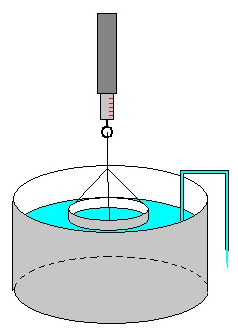
\includegraphics[width=0.8\textwidth]{Captura.PNG}
    \captionof{figure}{Diagrama anillo Du Nouy}
    \label{fig}
\end{Figura}

El método del anillo de du Nouy es una técnica para medir la tensión superficial de un líquido. El método consiste en levantar lentamente un anillo completamente sumergido de la superficie de un líquido. La fuerza $F$, requerida para levantar el anillo de la superficie del líquido se mide y se relaciona con la tensión superficial del líquido, $\eta$. La tensión superficial del líquido se calcula a partir del radio $r$ del anillo y del valor de la diferencia de fuerzas $F$ que mide el "dinamómetro"[2]:


\begin{equation}
    \eta = \frac{F}{4\pi r} \times 10^{5}
\end{equation}

con $r$ en $\text{cm}$ y $F$ en $\text{N}$ ($[\eta] = \frac{\text{dina}}{\text{cm}}$).




\newpage


\section*{Desarrollo experimental}

\begin{Figura}
\centering
    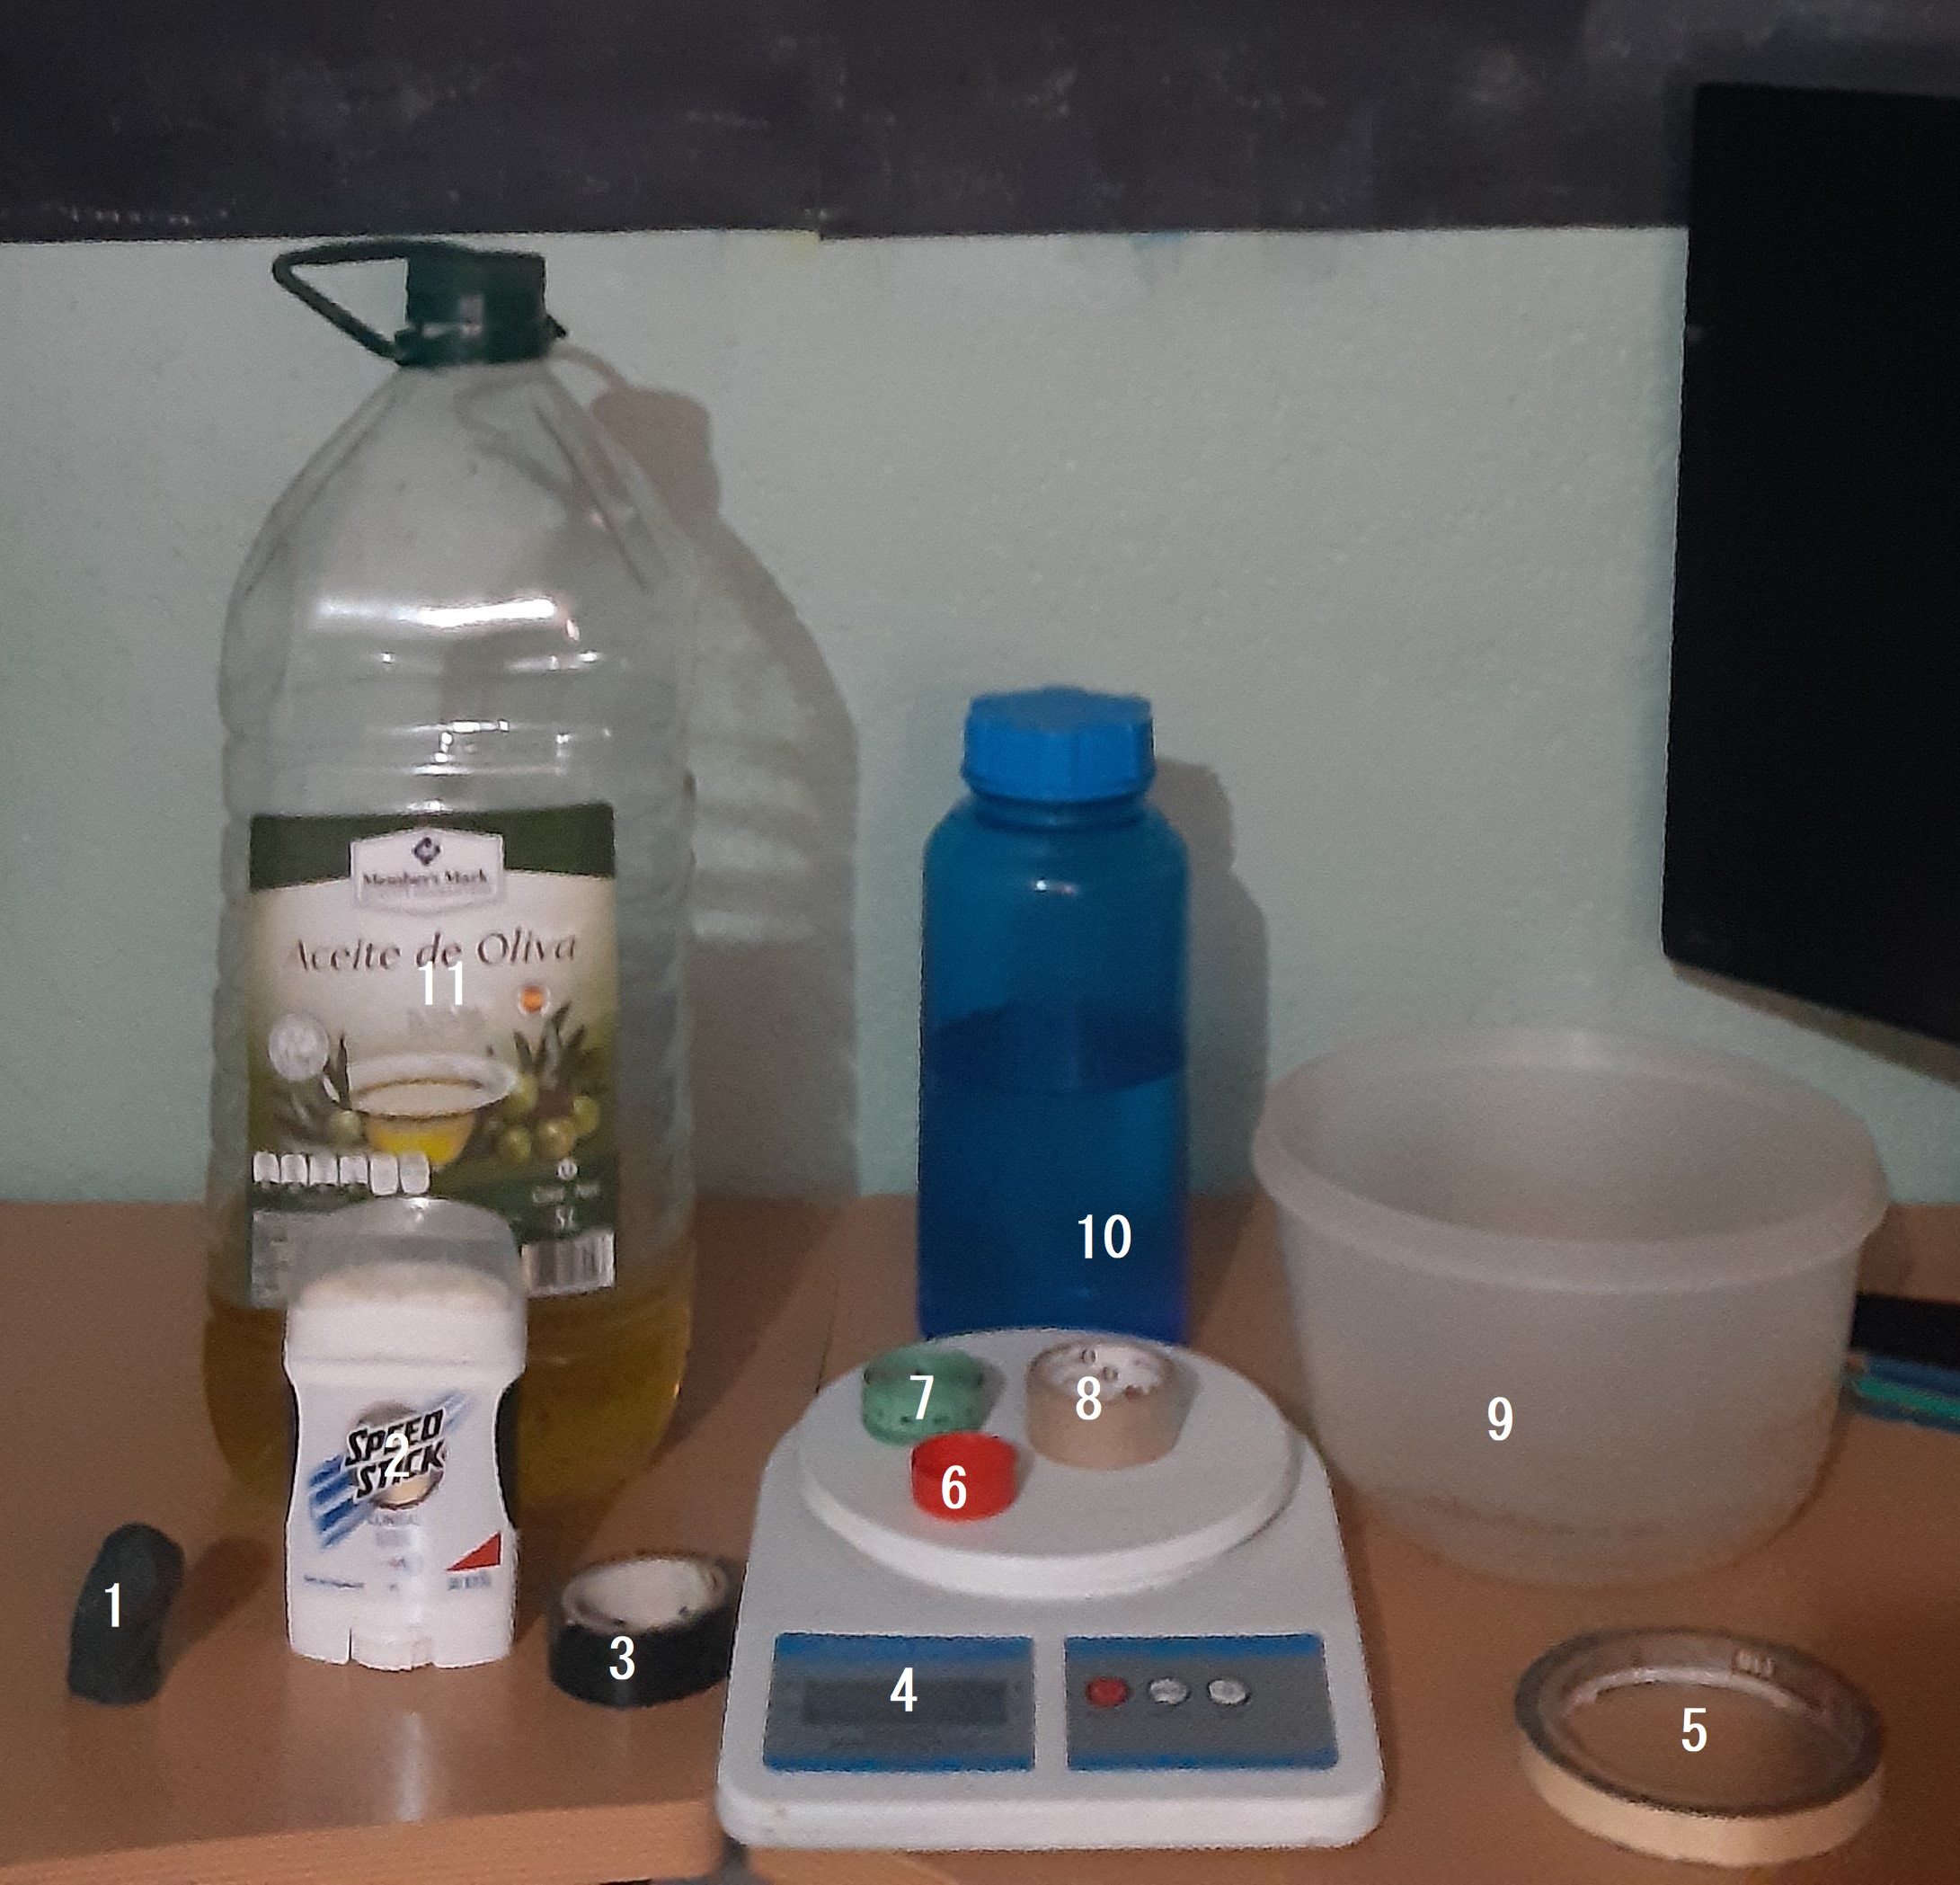
\includegraphics[width=0.8\textwidth]{20220428_143540.jpg}
    \captionof{figure}{Material: (1) Plastilina, (2) Desodorante en barra, (3) Hilo cáñamo, (4) Bascula digital, (5) Masquin tape, (6) Tapa de refresco, (7) Cinta métrica, (8) anillo, (9) Recipiente, (10) Agua, (11) Aceite de oliva.}
    \label{fig}
\end{Figura}

\begin{Figura}
\centering
    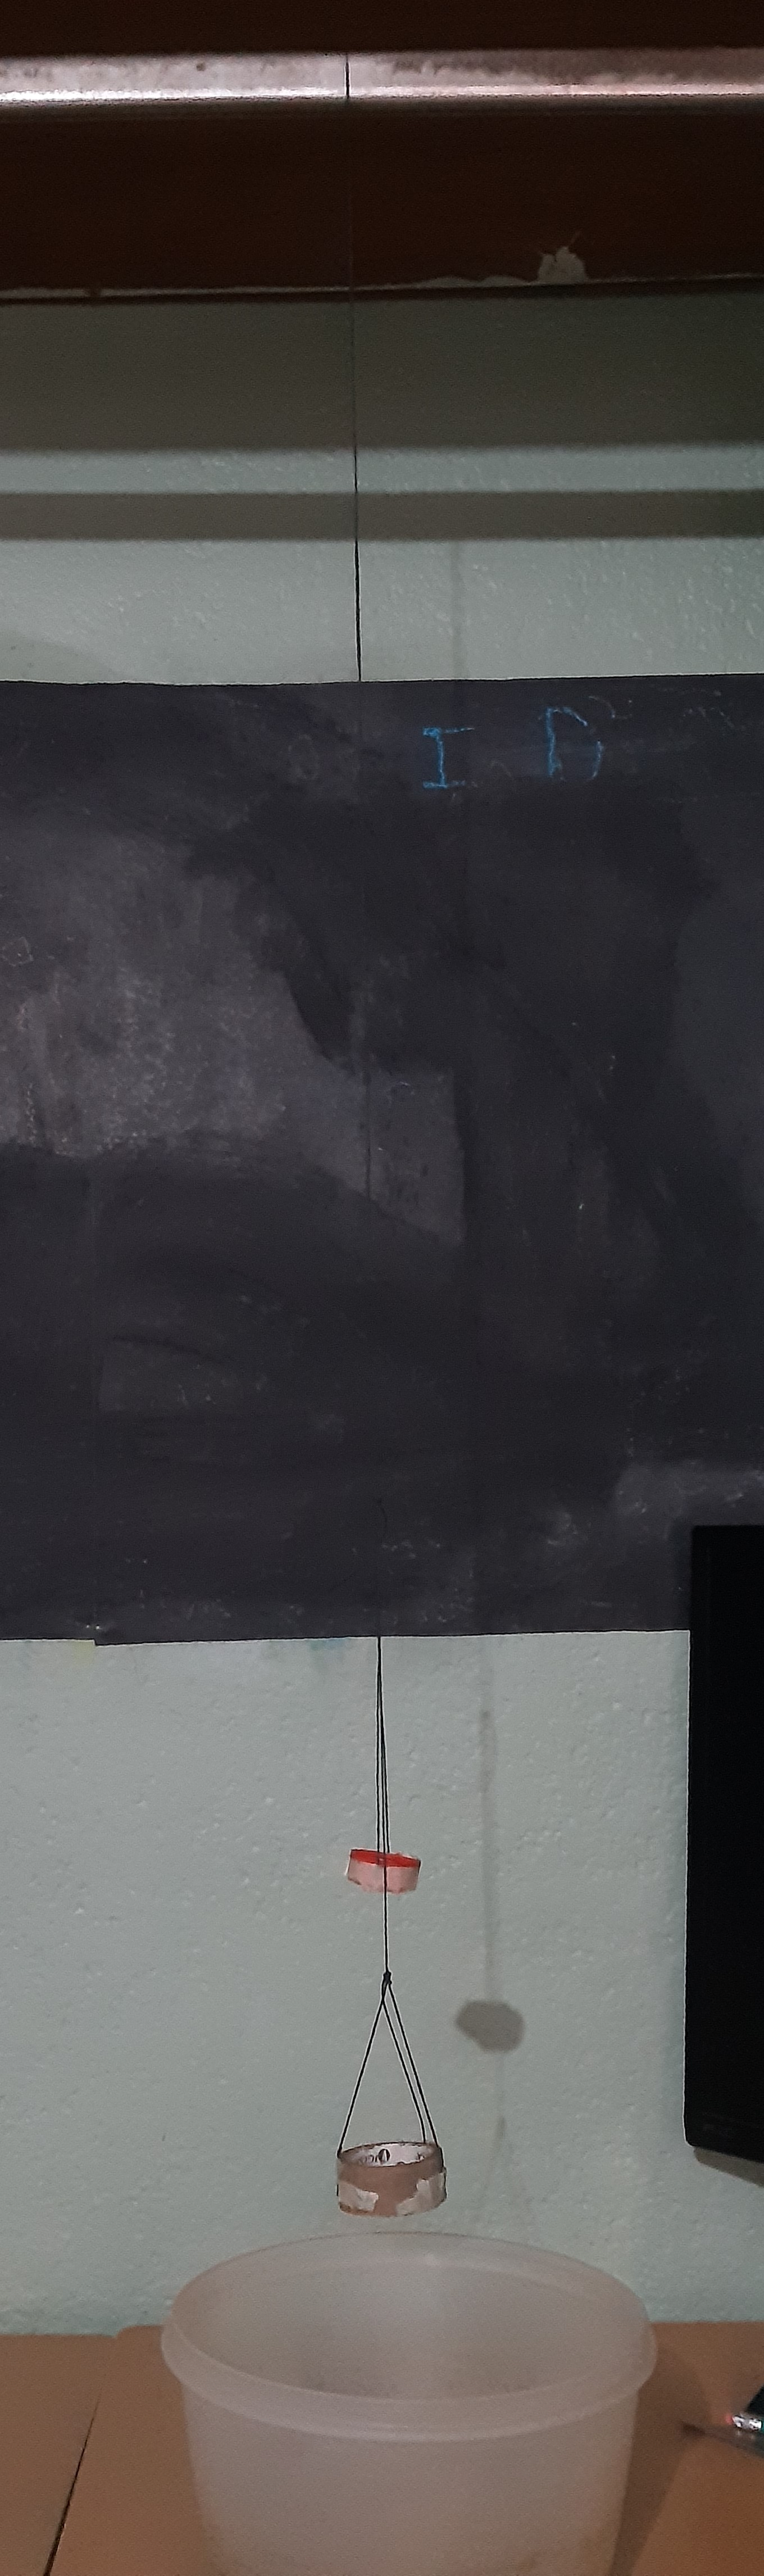
\includegraphics[width=0.5\textwidth]{20220428_164104.jpg}
    \captionof{figure}{Arreglo experimental.}
    \label{fig}
\end{Figura}

Se midió la masa y el radio medio del anillo con la bascula digital y la cinta métrica, se decidió empezar con el agua por lo que se llenó el recipiente con agua para después cortar un trozo de hilo cáñamo de aproximadamente metro y medio y con el masquin tape se pegó en un extremo del hilo la tapa de refresco de forma que se pudiera poner plastilina en su interior sin que esta se cayera, el otro extremo se pegó el anillo como se muestra en la figura 2. 

Con el desodorante en barra se lubricó una parte de un tubo para colgar ropa para colocar ahí el hilo con la tapa y el anillo y reducir la fricción, sobre el arreglo anterior se colocó el recipiente con agua y se introdujo por completo el anillo en el agua, se añadió poco a poco plastilina hasta que el anillo saliera por completo del agua y se midió la masa de la tapa y la plastilina usada. Se siguieron los mismo pasos para el aceite.




\section*{Resultados y Análisis}

\subsection*{Agua}

La fuerza ejercida sobre una masa $m$ en presencia de una gravedad $g$ es $F= mg$, la gravedad que se usará es $g = 9.8 \frac{\text{m}}{\text{s}^2}$.

Las masas medidas son:

\begin{equation*}
    m_{\text{anillo}}  = (0.006 \pm 0.00005)  \text{ kg} 
\end{equation*}

\begin{equation*}
     m_{\text{tapa}} = (0.010 \pm 0.00005) \text{ kg} 
\end{equation*}

entonces la diferencia de fuerzas es:

\begin{equation*}
    F= (m_{\text{tapa}} - m_{\text{anillo}})g = (0.0392 \pm 0.0098) N
\end{equation*}

El radio medido del anillo es:

\begin{equation*}
    r = (3.2 \pm 0.2) \text{ cm}
\end{equation*}

Entonces al propagar la incertidumbre en la ecuación (1) y sustituir, obtenemos una tensión superficial de:

\begin{equation*}
    \Delta \eta = \frac{1 \times 10^{5}}{4\pi}\sqrt{\left(\frac{\Delta F}{r}\right)^{2} + \left(\frac{F\Delta r}{r^2}\right)^{2}}
\end{equation*}

\begin{equation*}
    \eta_{\text{agua}} = (97.5 \pm 22.2) \frac{\text{dina}}{\text{cm}}  
\end{equation*}

en la literatura se reporta una tensión superficial para el agua de $72.3 \frac{\text{dina}}{\text{cm}}$.
\subsection*{Aceite de Oliva}

La masa medida de la tapa es:

\begin{equation*}
     m_{\text{tapa}} = (0.008 \pm 0.00005) \text{ kg} 
\end{equation*}

entonces la diferencia de fuerzas es:

\begin{equation*}
    F= (m_{\text{tapa}} - m_{\text{anillo}})g = (0.0196 \pm 0.0098) N
\end{equation*}

Entonces al propagar la incertidumbre en la ecuación (1) y sustituir, obtenemos una tensión superficial de:


\begin{equation*}
    \eta_{\text{aceite}} = (48.7 \pm 15.8) \frac{\text{dina}}{\text{cm}}  
\end{equation*}

en la literatura se reporta una tensión superficial para el aceite de oliva de $32 \frac{\text{dina}}{\text{cm}}$.

\section*{Conclusiones}

Las tensiones superficiales obtenidas se pueden considerar satisfactorios aún con el arreglo experimental casero ya que las discrepancias para el agua y el aceite son de $1.14$ y $1.06$ veces sus incertidumbres y con incertidumbres relativas de $23\%$ y $32\%$ respectivamente ($<2$).
  
\begin{thebibliography}{99}
\bibitem{1} Sears, Zemansky Física universitaria Vol. 1, Gpo.
Edit. Pearson Educación, 12 ed.l, México, 2009.


\bibitem{1} Tensión superficial en Los Líquidos. Mayo 8, 2022. http://www.sc.ehu.es/sbweb/fisica3/fluidos/tension
/tension.html.
\end{thebibliography}



\end{multicols}
\newpage

\section*{Apéndices}

\subsection*{Dinamómetro}

El dinamómetro es un instrumento utilizado para medir fuerzas o para calcular el peso de los objetos. El dinamómetro tradicional, inventado por Isaac Newton, basa su funcionamiento en el estiramiento de un resorte que sigue la ley de elasticidad de Hooke en el rango de medición. Al igual que una báscula con muelle elástico, es una balanza de resorte, pero no debe confundirse con una balanza de platillos (instrumento utilizado para comparar masas).

\begin{Figura}
\centering
    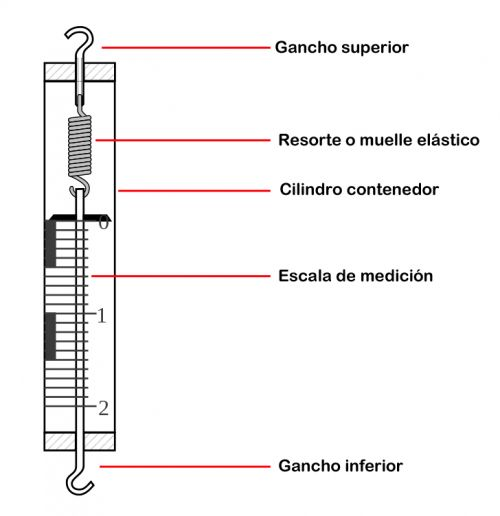
\includegraphics[width=0.5\textwidth]{dina_bg.jpg}
    \captionof{figure}{Esquema dinamómetro.}
    \label{fig}
\end{Figura}

Estos instrumentos constan de un muelle, generalmente contenido en un cilindro que a su vez puede estar introducido en otro cilindro. El dispositivo tiene dos ganchos o anillas, uno en cada extremo. Los dinamómetros llevan marcada una escala en el cilindro hueco que rodea el muelle. Al colgar pesos o ejercer una fuerza sobre el gancho exterior, el cursor de ese extremo se mueve sobre la escala exterior, indicando el valor de la fuerza.

\subsection*{Video}

https://drive.google.com/file/d/1LrNE8gmmKuIfwYihHjgKm0uq23sXSjLx/view?usp=sharing

\end{document}